\subsection{Project Budget} \label{sec:budget}
\noindent The table above shows the budget for FORWARD. As we continue to research and develop, there will likely be changes made to this table. The project will require a pre-built walker as well as 5 peripheral components, 2 motors, and 2 controllers, as well as wiring and PCB housing. \\

\begin{figure}[H]
	\centering
	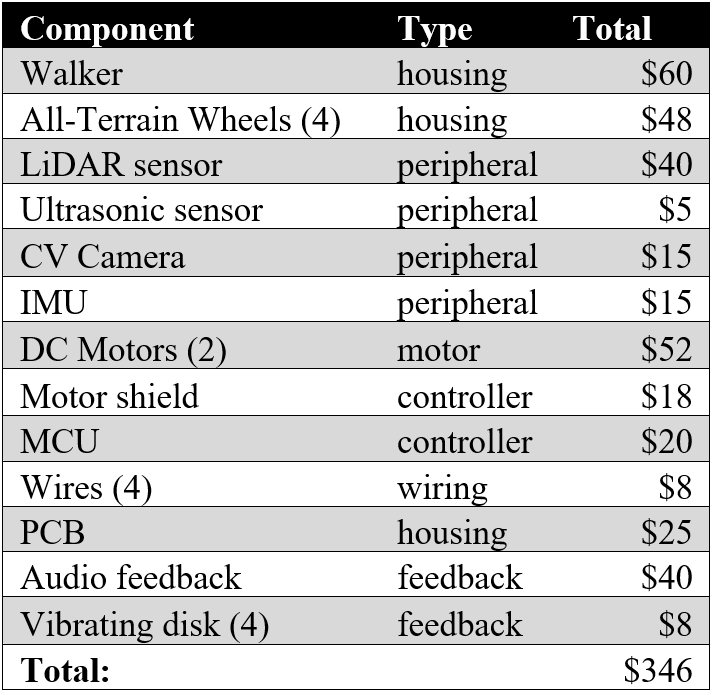
\includegraphics[width=0.5\textwidth]{./Images/Budget.png}
	\caption{\label{fig:Budget}Project Budget}
\end{figure}

\subsection{Project Bill of Materials} \label{sec:BOM}
\noindent Up to this point, the budget for sensors, processors, and motors has been successfully upheld. As advised by Dr. Wei early on to search Craig's List for a rollator, so we did and have found a great deal by a local close to UCF! Below are the expenditures to this point. We have yet to order PCB's at the time of submitting this document. Integration costs will inevitably come in senior design II.

\begin{figure}[H]
	\centering
	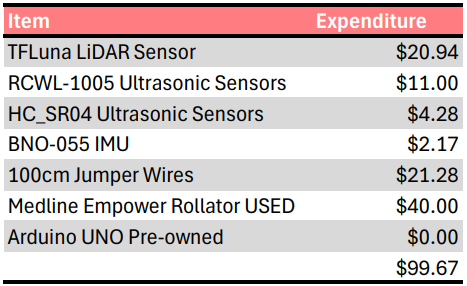
\includegraphics[width=0.5\textwidth]{./Images/detect-bom.png}
	\caption{\label{fig:detect-bom}Detection Subsystem Expenditures}
\end{figure}

\begin{figure}[H]
	\centering
	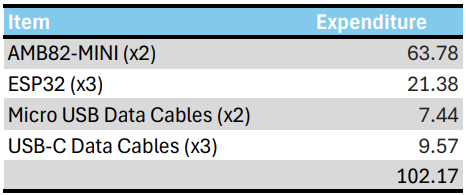
\includegraphics[width=0.5\textwidth]{./Images/identify-bom.png}
	\caption{\label{fig:identify-bom}Identification Subsystem Expenditures}
\end{figure}

\begin{figure}[H]
	\centering
	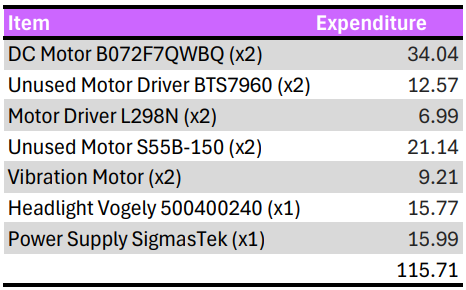
\includegraphics[width=0.5\textwidth]{./Images/avoid-bom.png}
	\caption{\label{fig:avoid-bom}Avoidance Subsystem Expenditures}
\end{figure}